\cotefile{57}
\scanpage{226}

Schémas de Picard des schémas formels en car. 0, \unsure{ou|où} des schémas propres sur une algèbre analytique sur $\mathbb{C}$

\margin{225}

\scanpage{227}

\begin{flushright}Neuilly July 6 1962\end{flushright}

Dear Hironaka,

I had a little thought over our conversation last tuesday, it occured to me that the type of argument I used yields in fact the following stronger result:

\uline{Theorem} Let $f:X\quad Y$ be a proper morphism of analytic spaces over $\underline{C}$, let $y\quad Y$, $Y_n=\operatorname{Spec\ an}(\underline{O}_y/\underline{m}_y^{n+1})$, $X_n=X\times_Y Y_n$,
\[
\begin{aligned}
\operatorname{Pic}(X_{\unsure{y}})&=R^1f(\underline{O}_X^{\bullet})_y=\underset{U\ni y}{\varinjlim}\operatorname{Pic}(f^{-1}(U)),\\
\operatorname{Pic}(\widehat{X}_y)&=\varprojlim\operatorname{Pic}(X_n).
\end{aligned}
\]
and consider the canonical homomorphisms
\diagram{\begin{tikzcd}
\operatorname{Pic}(X_y) \arrow[r,"u"] & \operatorname{Pic}(\widehat{X}_y) \arrow[r,"v_n"] & \operatorname{Pic}(X_n)
\end{tikzcd}}
Then the following are true:

(i) The inverse system $(\operatorname{Pic}(X_n))_{n\ \underline{N}}$ satisfies the condition of Mittag-Leffler (even with Artin-Riesz type of uniformity).

(ii) $\operatorname{Im}v_n=\operatorname{Im}v_nu={}$ (in virtue of (i)) set of universal images of $\operatorname{Pic}(X_n)$ in the inverse system $(\operatorname{Pic}(X_m))_{m\ \underline{N}}$.

(iii) In order for $u$ to be an isomorphism, it is nec and suff that $R^1f_*(\underline{O}_X)$ has a support not containing $y$ or having $y$ as an isolated point, i.e. $R^1f_*(\underline{O}_X)_y$ is a module of finite length.

In fact (i) can be made more precise:

(i bis) In the inverse system $(\underline{\operatorname{Pic}}_{X_n/\underline{C}})_{n\ \underline{N}}$ of analytic groups, the system of the ``Néron-Sévéri groups'' is constant for $n$ large, whereas for $m>n$ and $n$ large, the Kernel and Cokernel of
\diagram{\begin{tikzcd}
\underline{\operatorname{Pic}}_{X_m/\underline{C}} \arrow[r] & \underline{\operatorname{Pic}}_{X_n/\underline{C}}
\end{tikzcd}}
are just vector groups.

\margin{226}

\scanpage{228}

Parts (i) and (ii) yield the

\uline{Corollary 1} The following conditions are equivalent:

(i) There exists an open $U\quad y$ such that $X\ U$ is projective over $U$

(ii) For every $n$, $X_n$ is a projective analytic space.

For instance, if $\dim X_0\leq 1$, then (ii) and hence (i) holds.

The proof of the theorem only uses Grauerts analogues of the algebraic theorems of finiteness and comparison for direct images (cf his blue paper) and the usual exact sequence $0\quad\underline{Z}\quad\underline{O}\quad\underline{O}^{\bullet}\quad0$, together with some standard use of Mittag-Leffler story and five lemma. It is valid in fact for any $H^i(\underline{O}^{\bullet})$, not only $i=1$ (which seems the only one however to have geometric significance).

In the case of a \uline{formal} scheme propr over a complete noeth. local ring with residue field of \uline{caracteristic} 0, the analogon of the previous theorem (reducing to statements (i), (i bis)) \deleted{\unsure{(iii))|(iii)}} hold true, and I wrote a purely algebraic proof of this, relying only on the fact that the Kernel and Cokernel of $\underline{\operatorname{Pic}}_{X_{n+1}}\qquad\underline{\operatorname{Pic}}_{X_n}$ are without torsion, and Néron's finiteness theorem; in particular, the analogon of corollary 1 holds true in this case. These results break down of course in car. $>0$.

However, using the (as yet unwritten !) Gaga of Serre-Grauert-Remmert-Grothendieck (cf Grauert-Remmerts paper, complemented by the method of an old talk of mine in Cartan's Seminar, to recover the case of proper morphisms of \unsure{shhemes} from the projective one, via Chow's lemma \ldots), the analytic theorem above yields an interesting intrinsic property of analytic algebras over $\underline{C}$, with respect to algebraic geometry

\margin{227}

\scanpage{229}

over such an local ring:

\uline{Theorem} Let $A$ be an analytic algebra over $\underline{C}$ (we can suppose $A$ to be the ring of convergent power series\deleted{\unsure{)}} in $n$ variables), $\widehat{A}$ its completion, $Y$ and $\widehat{Y}$ the spectra, $X$ a proper scheme over $Y$, $\widehat{X}=X\times_Y\widehat{Y}$. Then:

(i) The inverse system $(\operatorname{Pic}(X_n))$ satisfies MLAR (as stated above, this depends only on the car. 0 assumption for the residue field).

(ii) $\operatorname{Pic}(X)$ and $\operatorname{Pic}(\widehat{X})$ have same image in $\unsure{\operatorname{Pic}}(X_n)$, - namely the group of ``universal images''. (NB recall $\operatorname{Pic}(\widehat{X})\simeq\varprojlim\operatorname{Pic}(X_n)$).

(iii) In order for $\operatorname{Pic}(X)\longrightarrow\operatorname{Pic}(\widehat{X})$ to be an isomorphism, it is necessary and sufficient that $\operatorname{supp}R^1f_*(\underline{O}_X^{\deleted{\unsure{\bullet}}})\subset(y)$, i.e. $H^1(X,\underline{O}_X)$ of finite length over $A$. (NB It amounts also to the same to \deleted{\unsure{impo}} ask that the inverse system of the subgroups $\operatorname{Pic}'(X_n)$ of universal images is constant for large $n$).

We get for example:

\uline{Corollary} 1 The following conditions are equivalent: (i) $X/Y$ projective (ii) $\widehat{X}/\widehat{Y}$ projective (iii) For every $n$, $X_n/Y_n$ projective.

This applies for instance if $\dim X_0\leq1$.

Now, applying your theorem of \uline{resolution of singularities}, and Mumford's method of relating the local Picard group of $A$ to the global Picard group of a regular scheme dominating $A$ birationally, one gets from the last statement \deleted{\unsure{in}} (iii) of last theorem:

\uline{Corollary} 2. Let $A$ be as above, assume \deleted{\unsure{the closed point $y$ of $Y$ to}} $Y'=Y-(y)$ regular, and let $\widehat{Y}'=\widehat{Y}-(\widehat{y})$. Then $\operatorname{Pic}(Y')\longrightarrow\operatorname{Pic}(\widehat{Y}')$ is an isomorphism\deleted{\unsure{?}}.

This explains ``à priori'' (when $A$ is normal) why Mumford was

\margin{228}

\scanpage{230}

\inserted{able} to introduce \deleted{(at least for \unsure{dim $d$|dim $2$}} on the group of divisor-classes of $A$ a structure of an analytic group (which in fact is algebraic\ldots), which from the algebraic point of view should be possible rather for the group of divisor classes of the completion $\widehat{A}$; of course Mumford uses directly the same kind of argument I used.

I do not know if in the last statement, the hypothesis that $Y'$ is regular (``$y$ isolated singularity'') is essential; we could dispense with it (\deleted{if you} and replace it simply by ``$A$ reduced'' if you can prove by your theory of resolution the following: if $f:X\rightarrow Y$ is proper ``birational'', $X$ regular, then $R^1f_*(\underline{O}_X)=0$. I understand you proved this if $Y$ also is regular (which is easily checked by your theory), but I wonder if this \uline{is really} needed.\margin{of course it is} I would not be surprised either if in this statement, $Y'$ can be replaced by any open subset of $Y$ (replacing of course $\widehat{Y}'$ by the inverse image of the latter). Moreover, I would expect the analogous statements to hold for $\pi_1$, more generally for all ``topological'' invariants as Weil homology, homotopy groups etc, that can be defined for schemes. \deleted{This}\inserted{This} should be related to the fact that all these invariants vanish for the geometric fibers of the morphism $\operatorname{Spec}(\widehat{A})\quad\operatorname{Spec}(A)$. This is easy to check at least for $\pi_0$ (and is true in fact for any henselian ring which is a ``good'' ring); however I do not know if this is true also for $\pi_1$.

Besides, I would not be surprised if most of the previous results (namely parts (ii) and (iii) of the second theorem, and the two corollaries, as well as the \deleted{previous} conjectures of the previous section) did hold true for any ``good'' ring which is henselian, \inserted{or} at least for the

\margin{229}

\scanpage{231}

``henselian closures'' of the local rings arising from algebras of finite type over a field, or over the integers, - although I do not have any result along these lines (except \inserted{those} stemming from my remark on $\pi_0$). \deleted{\unsure{For corollary}} This can be stated of course directly in terms of conjectures for the latter local rings without explicit reference to a henselian closure, for instance corollary 2 would yield the conjectural statement: Let $A$ be a local \deleted{\unsure{rin}} ring of an algebra of finite type over a field, $\widehat{A}$ its completion, $Y$ and $\widehat{Y}$ the spectra, $Y'$ and $\widehat{Y}'$ the complements of the closed points, \deleted{\unsure{i}} then any invertible sheaf on $\overset{\deleted{\unsure{\wedge}}}{\widehat{Y}'}$ can be defined by an inver\deleted{\unsure{si}}tible sheaf on some $Y_1'$, where $Y_1$ is local and $Y_1\quad Y$ is étale with trivial residue field extension (i.e. inducing an isomorphism for the completions in $A\quad A_1$). I wonder what information is given by Mumfords example in his blue paper, p.16, which I believe yields a case where the invertible sheaf considered does not come from an invertible sheaf on $Y'$ ? I \deleted{did} was not able to understand his construction.

Anyhow, one should be able to determine whether or not \deleted{\unsure{an}}\inserted{the} analytic algebras over $\underline{C}$ have any significant intrinsic property which is not shared by all ``good'' henselian rings with residu field of car. 0 (I recall that by good I mean ``quotient of a regular local ring $B$ such that the fibers of $\operatorname{Spec}\widehat{B}\rightarrow\operatorname{Spec}(B)$ are universally regular).

Please give my regards to Waka, and also Mireille's ; she just got the parcel from Waka, and was extremely pleased, in fact, she slipped into her new bed-shirt on the spot, and is delighted by it in every respect.

Sincerely yours

\margin{230}

\scanpage{233}

\margin{\fbox{\begin{tabular}{c}\uline{Pic d'un schéma formel}\\\uline{en car 0}\end{tabular}}}

\uline{Lemme} Soit $\varphi:G\mathbin{\text{---}}H$ \unsure{un hom} de type fini de groupes loc. de type fini sur un corps $k$. Alors

(i) $\underline{\pi}_0(\varphi):G/G^0\longrightarrow H/H^0$ est de type fini, en particulier son noyau est fini.

\margin{(Donc si $H/H^0$ est \unsure{à engendrement} fini, il en est de $=$ de $G/G^0$)}

\deleted{[Si $N=\operatorname{Ker}\varphi$ est connexe, alors $\underline{\pi}_0(\varphi)$ est $\unsure{\simeq}$ une immersion fermée]}

(ii) Supposons que $N=\operatorname{Ker}\varphi$ soit \uline{connexe}, \unsure{soit} $H'=\operatorname{Im}\varphi$, \inserted{$i:H'\rightarrow H$ l'imm. can.} Alors $\operatorname{Ker}\underline{\pi}_0(\varphi)$\inserted{, $\operatorname{Coker}\underline{\pi}_0(\varphi)$ et $\operatorname{Coker}\varphi$ ne changent}
\deleted{$\simeq\operatorname{Ker}\underline{\pi}_0(i)\simeq(H'/H'^0)\cap(H/H'^0)^0$.}
quand on remplace $(G,H,\varphi)$ par $(H',H,i)$ ou encore par $(\underbrace{H'/H'^0}_{\inserted{\text{discret }\unsure{\in|\subset}F}},H/H'^0,i')$ \unsure{\ldots}.

\deleted{\uline{Corollaire}} \inserted{(iii)} Supposons \inserted{$\operatorname{Ker}\varphi$ soit connexe et} que $\operatorname{Coker}\varphi$ soit ``\unsure{géom\textsuperscript{t}} sans torsion''. Alors $\underline{\pi}_0(\varphi)$ est injectif et $\operatorname{Coker}\underline{\pi}_0(\varphi)$ est sans torsion.

Dém\inserted{de (iii)}. Grâce à \unsure{(ii)} précédent, on est ramené au cas où $\varphi$ est une imm fermée, et où $G$ est \unsure{discret géom.} Mais alors $\operatorname{Coker}\varphi$ contient $H^0/G\cap H^0$ où $G\cap H^0\simeq\operatorname{Ker}\underline{\pi}_0(\varphi)$. Si ce \unsure{quotient} est sans torsion, il faut que, ou bien

\margin{232}

\scanpage{234}

\uline{ALGEBRE COMMUTATIVE}
\margin{Rédaction\\n\textsuperscript{o}336}

\uline{Fascicule I}

CHAPITRE IV : DECOMPOSITION PRIMAIRE

\diagram{\begin{tabular}{p{12cm}r}
 & n\textsuperscript{o} des pages\\
\S 1. Idéaux premiers associés à un module & \\
1. Définition des idéaux premiers associés \dotfill & 1\\
2. Localisation des idéaux premiers associés \dotfill & 3\\
3. Relations avec le support \dotfill & 5\\
4. Cas des modules de type fini \dotfill & 6\\[1ex]
\S 2. Décomposition primaire & \\
1. Sous-modules primaires \dotfill & 8\\
2. Existence d'une composition primaire \dotfill & 10\\
3. Propriétés d'unicité dans la décomposition primaire \dotfill & \uline{11}\\
4. Localisation d'une décomposition primaire \dotfill & 12\\
5. Anneaux et modules de longueur finie \dotfill & 13\\[1ex]
\S 2. Cas des modules gradués \dotfill & \unsure{18|16}
\end{tabular}}

\margin{\figure{\begin{tikzpicture}[x=1cm,y=1cm]
\draw (0,5.7) .. controls (.45,5.65) and (.55,5.35) .. (.55,5.05) -- (.49,.75);
\draw (-.12,.3) .. controls (.1,.37) and (.32,.31) .. (.39,.34) .. controls (.16,.4) and (.06,.25) .. (-.1,.25);
\draw (-.31,.34) -- (-.22,.33);
\end{tikzpicture}}}

\begin{center}\texttt{-:-:-:-}\end{center}

\margin{233}

\scanpage{235}

a) $\operatorname{car}k>0$, \deleted{\unsure{alors} $H^0$ fini} \inserted{et} $H^0$ \deleted{\unsure{est}} réduit à un pt; alors $G\cap H^0=\{e\}$ i.e. $\underline{\pi}_0(\varphi)$ est injectif, et du pt de vue géométrique \unsure{ensembliste} on a $\varphi=\underline{\pi}_0(\varphi)$ donc $\operatorname{Coker}\underline{\pi}_0(\varphi)$ est sans torsion

b) $\operatorname{car}k=0$, $H^0$ est un groupe \uline{vectoriel}, \deleted{\unsure{et}} donc le sous-grp fini $G\cap H^0=0$.
\margin{$G\subset H$}
D'où \deleted{\unsure{il}} on a une \unsure{s.e.} exacte
\diagram{\begin{tikzcd}
0 \arrow[r,no head] & H^0 \arrow[r] & H/G \arrow[r] & \unsure{\operatorname{Coker}\underline{\pi}_0(\varphi)} \arrow[r] \arrow[d,equal] & 0\\
 & & & H/(G+H^0) &
\end{tikzcd}}
qui \unsure{splitte} du pt de vue géométrique ensembliste (car $\unsure{H^0_{\bar{k}}|H^0}$ est divisible). Comme $H/G$ est sans torsion, il en est donc de $=$ de $\operatorname{Coker}\underline{\pi}_0(\varphi)$.

\uline{Corollaire 1} Soit $(G_n)_{n\in\unsure{\mathbf{Z}|\mathbf{N}}}$ un syst projectif de groupes \deleted{\unsure{alg.}}\inserted{comm} loc. de type fini sur le corps $k$. Supposons

\inserted{a) \deleted{\unsure{Si}} $G_0/G_0^0$ est à engendrement fini}

\inserted{\unsure{b)}} que pour tout $n$, l'hom de transition
\diagram{\begin{tikzcd}G_{n+1}\arrow[r]&G_n\end{tikzcd}}
\deleted{\unsure{ait}}\inserted{est de type fini et} a un noyau connexe, et un conoyau qui est géométriquement \uline{sans} torsion.

\inserted{b) pour $\forall n$, $\underline{\pi}_0(G_n)$ est à engendrement fini.}

\margin{234}

\scanpage{236}
\mspage{17}
\margin{n\textsuperscript{o} 227}

des points fixes.

PROPOSITION 1. - \uline{Soit $\mathcal{L}$ un système linéaire sans composante fixe, et $T$ l'application rationnelle associée. Soit $P'$ un point normal de $V$. Alors $T$ est définie en $P'$ si et seulement si $P'$ n'est pas un point de base.}

\uline{Dém.} Supposons que $P'$ ne soit pas un point de base. Soit $Y=\sup$ des pôles des $f_i$, et écrivons $(f_i)=X_i-Y$. Alors par hypothèse, il existe un index $i$, mettons $i=0$, tel que $P'\notin|X_0|$. On a $(f_i/f_0)=X_i-X_0$. Par la prop. 5 du \S 1, chaque fonction $f_i/f_0$ n'a pas de pôle passant par $P'$, et est définie en $P'$. La réciproque est également claire.

Soit $\mathcal{L}$ un système linéaire sans composante fixe, et $T:V\longrightarrow V'$ l'application rationnelle induite par $\mathcal{L}$. On va voir que $T$ applique les diviseurs de $\mathcal{L}$ sur les \inserted{\unsure{sections}} \unsure{hyperplans|hyperplanes} de $V'$ de la manière suivante. Prenons $X\in\mathcal{L}$, $P'\in|X|$ et supposons que $P'$ ne soit pas un point de base pour $\mathcal{L}$. Prenons un diviseur $X_0\in\mathcal{L}$ tel que $P'\notin|X_0|$. Soit $L_0$ l'espace dérivé de $\mathcal{L}$ par $X_0$ et $f_0,\ldots,f_n$ une base de $L_0$. Alors chaque fonction $f\in L_0$ peut être écrite
\[
f=f_c=\sum c_i f_i\qquad c_i\in k
\]
et $(f_c)=X_c-X_0$. Supposons $X=X_c$. Puisque $P'\notin|X_0|$, toutes les fonctions $f_i$ sont définies en $P'$. Mais $P'\in|X_c|$ implique que $\sum c_i f_i(P')=0$, i.e. $T(P')$ est dans l'hyperplan définit par l'équation $\sum c_i X_i=0$.

Un système linéaire sera dit \uline{ample} \inserted{s'il est sans \unsure{com.|comp.} fixe et} si l'application rationnelle $T$ induite par $\mathcal{L}$ est un isomorphisme de $V$ sur $V'$. Si $D$ est un diviseur tel que $\mathcal{L}(D)$ soit ample, alors $D$ est dit \uline{ample}. Le système des

\margin{235}

\scanpage{237}

Dans ces conditions

(i) Le système projectif $(\underline{\pi}_0(G_n))_n$ est essentiellement constant.

(ii) Les systèmes $(G_n^0)_n$ (donc aussi le système $(G_n)$) \unsure{satisfont|satisfait} (M.L.).

(iii) \deleted{P\unsure{our} \illegible{3}} \deleted{(\unsure{s.c.} \illegible{2})} $\exists n_0$ tq \deleted{et conoyau} que \unsure{pour|$\forall$} $m\geq n\geq n_0$, le \unsure{conoyau|noyau} de $G_m\longrightarrow G_n$ soit un groupe vectoriel \deleted{sans torsion (donc} en car $=0$, et \deleted{\unsure{purement}} radiciel en car. $>0$.

\deleted{\unsure{en car} \illegible{3}}

\inserted{Si la car. est nulle et si les \deleted{\unsure{connexes}} $\operatorname{Ker}(G_{n+1}\rightarrow G_n)$ sont unipotents, alors les noyaux des $(\unsure{G_m\rightarrow G_n})$ sont aussi vectoriels.}

\uline{Corollaire 2} Supposons que les $\operatorname{Ker}(G_m\rightarrow G_n)$ \inserted{pour $m\geq n$} soient \deleted{$=$}\inserted{de} plus des groupes \deleted{\unsure{commut.} vectoriels} linéaires \deleted{\unsure{résolubles}}\inserted{unipotents}, \deleted{supposons $k$ parfait} et supposons $k$ parfait [le cas important est $k$ de car. 0] Alors le système des $(G_n(k))_n$ satisfait ML

\margin{236}

\scanpage{238}

IV -- \mspage{9} -- \hfill n°338

que $\underline m^n\subset\underline q$ (Chap.III, §2, n°2, cor. 2 du lemme 2).

3) Dans un anneau \uline{principal} $A$, les idéaux primaires sont $(0)$ et ceux de la forme $(p^n)$ avec $p$ extrémal et $n\geq1$ : ceci résulte de l'ex. 2.

4) Les puissances d'un idéal premier quelconque $\underline p$ ne sont pas en général des idéaux primaires (exerc.\quad). Il existe des idéaux primaires qui ne sont pas des puissances d'idéaux premiers (exerc.\quad).

\margin{\unsure{2}}

PROPOSITION 2.- \uline{Soient} $M$ \uline{un module sur un anneau noethérien} $A$, $\underline p$ \uline{un idéal premier de} $A$, \uline{et} $(Q_i)_{i\in I}$ \uline{une famille finie non vide de sous-modules $\underline p$-primaires de} $M$. \uline{Alors} $\bigcap_{i\in I}Q_i$ \uline{est $\underline p$-primaire}.

En effet $M/\bigcap_{i\in I}Q_i$ est isomorphe à un sous-module non nul de la somme directe $\sum_{i\in I}M/Q_i$. Or $\operatorname{Ass}(\sum_{i\in I}M/Q_i)=\bigcup_{i\in I}\operatorname{Ass}(M/Q_i)=\{\underline p\}$ (§1, cor.1 de la prop. 3). Donc $\operatorname{Ass}(M/\bigcap_{i\in I}Q_i)=\{\underline p\}$ (§1, prop.3).

PROPOSITION 3.- \uline{Soient} $A$ \uline{un anneau noethérien}, $S$ \uline{une partie multiplicative de} $A$, $\underline p$ \uline{un idéal premier de} $A$, $M$ \uline{un $A$-module}, $N$ \uline{un sous-module} $M$, \uline{et} $i=i_M^S$ \uline{l'application canonique de} $M$ \uline{dans} $S^{-1}M$.

a) \uline{On suppose} $\underline p\cap S\neq\varnothing$. \uline{Si} $N$ \uline{est $\underline p$-primaire}, \uline{on a} $S^{-1}N=S^{-1}M$.

b) \uline{On suppose} $\underline p\cap S=\varnothing$. \uline{Pour que} $N$ \uline{soit $\underline p$-primaire}, \uline{il faut et il suffit que} $N$ \uline{soit de la forme} $i^{-1}(N')$, \uline{où} $N'$ \uline{est un sous-module $(S^{-1}\underline p)$-primaire de} $S^{-1}M$. \uline{On a alors} $N'=S^{-1}N$.

Si $\underline p\cap S\neq\varnothing$ et si $N$ est $\underline p$-primaire, on a $\operatorname{Ass}(S^{-1}(M/N))=\varnothing$ (§1, prop.5), donc $S^{-1}M/S^{-1}N=S^{-1}(M/N)=(0)$ (§1, cor.1 de la prop.2), et par conséquent $S^{-1}N=S^{-1}M$.

Supposons $\underline p\cap S=\varnothing$. Si $N$ est $\underline p$-primaire, on a $\operatorname{Ass}(S^{-1}(M/N))=\{S^{-1}\underline p\}$ (§1, prop.5), donc le sous-module $N'=S^{-1}N$ de $S^{-1}M$ est $(S^{-1}\underline p)$-primaire ; en outre, si $s\in S$ et $m\in M$ sont tels que $sm\in N$, on a $m\in N$ (car l'homothétie définie par $s$ dans $M/N$ est injective), d'où $N=i^{-1}(N')$ (Chap.II,

\margin{237}

\scanpage{239}

\margin{\unsure{$G_m$}$\longrightarrow$ \quad \unsure{$G_n$}$\longrightarrow$}

\margin{\diagram{\begin{tikzcd}[column sep=large]
\deleted{\unsure{P|R}}\arrow[r] & \deleted{Q}\arrow[r] & \deleted{R}
\end{tikzcd}}}
\margin{\deleted{$\operatorname{Im}\unsure{P}\cap\operatorname{Ker}(\unsure{Q})$}}
\margin{\deleted{$\operatorname{Im}(\unsure{P|R}\longrightarrow Q)\cap\operatorname{Ker}(Q\longrightarrow R)$}}

En effet, si $G_{m,n}=\operatorname{Im}(G_m\unsure{\longrightarrow|\text{---}}G_n)$ pour $m\geq n$, on sait que
\[
G_{m,n}(k)\unsure{=|\supset}\operatorname{Im}(G_m(k)\longrightarrow G_n(k))
\]
\unsure{par ce fait que} $\mathrm H^1(k,N_{m,n})=0$. Par suite, \inserted{pour $n$ fixé,} \unsure{la suite|les suites} des $\operatorname{Im}(G_m(k)\longrightarrow G_n(k))$ \unsure{sont|est} \unsure{stationnaires|stationnaire}.

N.B. En car. 0, \unsure{tout} groupe algébrique \unsure{commutatif} unipotent est connexe \inserted{et un gr \uline{vectoriel}}, donc si les $\operatorname{Ker}(G_{n+1}\longrightarrow G_n)$ sont des groupes \deleted{\unsure{vectoriels}}\inserted{unipotents}, \deleted{\unsure{$G_m$} \illegible{3}}\inserted{alors \deleted{et} les} \deleted{\unsure{les}} $\operatorname{Ker}(G_m\longrightarrow G_n)$ pour $m\geq\deleted{\unsure{n_0}}n$ \unsure{sont} des groupes vectoriels, en particulier connexes.

\margin{\unsure{voir ça}}
\figure{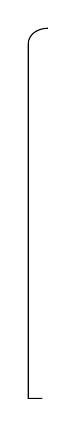
\begin{tikzpicture}[x=1cm,y=1cm]
\draw (0.18,0) -- (0,0) -- (0,4.5) to[out=90,in=180] (0.25,4.7);
\end{tikzpicture}}

\uline{Pr.} Soit $\mathfrak X$ un schéma formel \inserted{(propre)} sur un anneau local noethérien complet $A$, contenant un \uline{corps $k$ de car. 0} tel que \deleted{\unsure{le}} $k(A)$ soit fini sur $k$. Considérons les $X_n$ comme des schémas propres sur $k$, \deleted{Alors} considérons le syst. projectif
\[
(\underline{\operatorname{Pic}}_{X_n/k})
\]
Alors ce syst. \unsure{satisfait} aux conditions

\figure{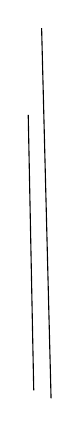
\begin{tikzpicture}[x=1cm,y=1cm]
\draw (0.12,0) -- (0,4.7);
\draw (-0.1,0.1) -- (-0.17,3.6);
\end{tikzpicture}}

\margin{238}

\scanpage{240}

IV -- \mspage{7} -- \hfill n°338

Avec les notations du th.2, l'ensemble $\{\underline p_0,\ldots,\underline p_{n-1}\}$ n'est pas nécessairement déterminé de façon unique par $M$ ; en particulier il peut être distinct de $\operatorname{Ass}(M)$.

PROPOSITION 8.- \uline{Soient} $A$ \uline{un anneau noethérien}, $\underline a$ \uline{un idéal de} $A$, \uline{et} $M$ \uline{un $A$-module de type fini}. \uline{Les conditions suivantes sont équivalentes} :

a) \uline{il existe un élément non nul} $x$ \uline{de} $M$ \uline{tel que} $\underline ax=(0)$,

b) \uline{pour tout} $a\in\underline a$, \uline{il existe un élément non nul} $x$ \uline{de} $M$ \uline{tel que} $ax=0$ ;

c) \uline{il existe} $\underline p\in\operatorname{Ass}(M)$ \uline{tel que} $\underline a\subset\underline p$.

Il est clair que a) implique b). D'après le cor. 2 de la prop.2, la condition b) signifie que $\underline a$ est contenu dans la réunion des idéaux premiers associés à $M$, donc dans l'un d'eux puisque $\operatorname{Ass}(M)$ est fini (Chap.II, §1, n°1, lemme 2) ; ainsi b) implique c). Enfin, s'il existe $\underline p\in\operatorname{Ass}(M)$ tel que $\underline a\subset\underline p$, $\underline p$ est l'annulateur d'un élément non nul $x$ de $A$ (déf.1), et on a $\underline ax=(0)$ ; donc c) implique a).

PROPOSITION 9.- \uline{Soient} $A$ \uline{un anneau noethérien}, $\underline a$ \uline{un idéal de} $A$, \uline{et} $M$ \uline{un $A$-module de type fini}. \uline{Pour qu'il existe un entier} $n>0$ \uline{tel que} $a^nM=(0)$, \uline{il faut et il suffit que $a$ soit contenu dans l'intersection des idéaux premiers associés à} $M$.

La condition est nécessaire en vertu du cor. de la prop.7. Réciproquement, ce même corollaire et le fait que $M$ est de type fini, montrent que tout élément $a$ de $\underline a$ définit une homothétie nilpotente de $M$ ; en particulier, si $(a_1,\ldots,a_n)$ est un système fini de générateurs de $\underline a$, il existe des entiers $n(i)>0$ tels que $a_i^{n(i)}M=(0)$ pour $1\leq i\leq q$ ; on a alors $\underline a^{n(1)+\cdots+n(q)}M=(0)$ ce qui termine la démonstration.

\begin{center}-:-:-:-\end{center}

\margin{239}

\scanpage{241}

du cor 1 précédent, et le système des $\underline{\operatorname{Pic}}_{X_{\unsure{n|0}}/k}(k)$ satisfait à M.L.

\margin{\figure{\begin{tikzpicture}
\node[draw,ellipse,rotate=25,align=left,inner sep=8pt] {\uline{N.B.} les\\\unsure{grs} $=$ \unsure{vérifient}\\M.L.A.R.};
\end{tikzpicture}}}

\uline{N.B.} On suppose l'existence des $\underline{\operatorname{Pic}}_{X_n/k}$. Elle est prouvée en général par \uline{Murre}. Dans le cas projectif, on le sait par Grothendieck -- Oort.

Le fait que les $\underline{\operatorname{Pic}}_{X_{n+1}/k}\longrightarrow\underline{\operatorname{Pic}}_{X_n/k}$ sont de type fini, \deleted{et} les noyaux \deleted{sans torsion} unipotents, les conoyaux sans torsion, se voit par la \unsure{thèse|théorie} de Oort \deleted{\unsure{et}} \deleted{des obstructions} [cf suite ex. de cohomologie]. De plus, on utilise le th. \inserted{de finitude} de Néron \deleted{\unsure{Séveri}} pour $\underline{\operatorname{Pic}}_{X_0/k}$.

\margin{(\unsure{des anneaux locaux artiniques|des anneaux locaux artiniens})}
\margin{(\unsure{locaux artiniques|locaux artiniens})}

\uline{Corollaire} \inserted{Soit $\mathfrak X$ préschém. \unsure{formel} propre sur un anneau local noeth. complet à corps résiduel $k$ de car. 0. Supposons que les comp. connexes de $X_0$ soient géomt. connexes et \unsure{admettent un pt rat/$k$}. Alors} le système projectif $(\operatorname{Pic}(X_n))_{n\in\unsure{\mathbf Z|\mathbf N}}$ satisfait à M.L.

\figure{\begin{tikzpicture}[x=1cm,y=1cm]
\draw (0,0) -- (0,1.1);
\end{tikzpicture}}

\margin{On \unsure{peut} supposer $k\subset A$ \unsure{grâce à Cohen}.}

\deleted{Lorsque les composantes connexes de $X_0$ sont géomt. connexes, et que \unsure{ces dernières} \unsure{admettent} un pt rat/$k$, cela \unsure{provient du}}
\inserted{\unsure{provient de}}

\margin{240}

\scanpage{242}

-- \mspage{16} -- \hfill n° 227

3. \uline{L'application rationnelle définie par un système linéaire}.

On continue à supposer $V$ complète. Soit $\mathcal L$ un système linéaire, $X_0\in\mathcal L$, et $L_0$ le module dérivé de $\mathcal L$ par $X_0$. Soit $f_0,\ldots,f_n$ une base de ce module. Alors les fonctions $(1,f_1/f_0,\ldots,f_n/f_0)$ peuvent être prises comme coordonnées non homogènes d'un point dans l'espace projectif, qui représente un point générique d'une variété projective $V'$. Si $t$ est un élément transcendant sur tout, alors $(tf_0,\ldots,tf_n)$ sont les coordonnées homogènes d'un point générique de $V'$. Elles définissent une application rationnelle $T:V\longrightarrow V'$ de $V$ sur $V'$. Un changement de base dans $L_0$ donne une transformation projective de $V'$.

Si on employait un module $L_1$ dérivé de $\mathcal L$ par un autre diviseur $X_1$, on voit que l'application rationnelle $T_1$ obtenue comme ci-dessus diffère de $T$ par une transformation \deleted{linéaire}\inserted{projective}. On peut donc dire que $T$ est uniquement déterminée par $\mathcal L$. De plus, si $\mathcal L$ et $\mathcal L'$ soit deux systèmes linéaires qui ne diffèrent que par une composante fixe, alors on voit immédiatement qu'ils donnent lieu à la même application rationnelle $T$ de $V$, les modules dérivés étant les mêmes. Pour étudier l'application rationnelle associée à un système linéaire, on peut donc se borner, sans perte de généralité, aux systèmes linéaires \unsure{sans'|sans} composantes fixes.

\figure{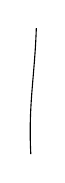
\begin{tikzpicture}[x=1cm,y=1cm]
\draw (0.07,1.6) to[out=-92,in=93] (0,0);
\end{tikzpicture}}

On va maintenant donner un critère pour que l'application rationnelle $T$ soit définie en un point $P$ de $V$.

Un point $P$ de $V$ est dit un \uline{point de base} du système linéaire $\mathcal L$ si $P\in\inserted{\unsure{\checkmark|\gamma}}|X|$ pour tout $X\in\mathcal L$. Si $Y$ est une composante fixe de $\mathcal L$, alors tous les points de $|Y|$ sont des points de base. Il peut très bien arriver qu'un système linéaire n'ait pas de composante fixe, mais ait

\margin{241}

\scanpage{243}

\[
\operatorname{Pic}(X_n)\xrightarrow{\sim}\underline{\operatorname{Pic}}_{X_n/k}(k)
\]
et du th. précédent. Dans le cas général, \unsure{Notons} \deleted{d'abord} \unsure{ceci|cas} [où $k'/k$ est une extension finie de $k$, \unsure{que l'on choisit} de façon

\deleted{\uline{Lemme} Sous les conditions du corollaire [car. 0 \unsure{essentielle}, mais non la \unsure{propreté}], le conoyau de $\operatorname{Pic}(X_m)\unsure{\text{---}|\longrightarrow}\operatorname{Pic}(X_n)$ (pour $m\geq n$) est sans torsion.}

\deleted{On est \unsure{ramené} au cas où $m=n+1$, où cela \deleted{\unsure{en}} résulte du fait que ce conoyau est $\subset\mathrm H^2(X_0,\deleted{\unsure{F_2}}\inserted{F^{(n)}})$, $F_{\deleted{\unsure{n}}}^{(n)}$ un Module \unsure{coh.} convenable sur $X_0$.}

pour \deleted{\unsure{le}} $X_0\otimes_k k'$ satisfasse \unsure{aux} conditions énoncées plus haut] : on a une suite exacte

\diagram{\begin{tikzcd}[column sep=large]
0\arrow[r] & \operatorname{Pic}(X_n)\arrow[r] & \underline{\operatorname{Pic}}_{X_n/k}(k)\arrow[r] & \check{\mathrm H}^{2}(k'/k,M_n)
\end{tikzcd}}

\margin{\uline{\unsure{rigoureux}??} \quad \uline{À \unsure{expliciter}}}
\figure{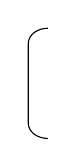
\begin{tikzpicture}[x=1cm,y=1cm]
\draw (0.25,0) to[out=180,in=-90] (0,0.2) -- (0,1.2) to[out=90,in=180] (0.25,1.4);
\end{tikzpicture}}

où $M_n$ est le schém. en groupes [comm. \unsure{lisse} connexe] \deleted{\unsure{tel}} qui décrit les unités de la $k$-algèbre \deleted{$\unsure{k_2}$} $\mathrm H^0(X_n,\mathcal O_{X_n})$. On voit que le système projectif des $(M_n)$ satisfait M.L. [groupes \deleted{alg. \unsure{connexes}}\inserted{\uline{de type fini} sur $k$ !}] et est à noyaux \deleted{\unsure{unipotents}} [\unsure{ici}, \uline{vectoriels}\ldots]

\margin{242}

\scanpage{244}

-- \mspage{15} -- \hfill n° 227

linéaire, le système des hypersurfaces de degré donné sur une variété projective.

Soit donc $V$ une variété projective, et $R=k[x]=k[x_0,\ldots,x_N]$ son anneau de coordonnées homogènes, comme dans IAG, ch.IV. Soit $I$ \deleted{la fermeture intégrale de $R$}, et $R_n$, $I_n$ les éléments homogènes de degré $n$ de $R$ et de $I$. Soit $f\in R_n$. On va associer un diviseur positif $Z(f)$ à $f$, qui sera appelé l'hypersurface section de $V$ par $f$. Soit $W^{r-1}$ un diviseur premier de $V$. Supposons que $W$ ne soit pas contenu dans l'hyperplan $X_0=0$. Alors $f(x)/x_0^n$ est une fonction $\varphi$ sur $V$. On définit la multiplicité de $W$ dans le diviseur $Z(f)$ comme étant $\operatorname{ord}_W\varphi$. (Il est clair que $\operatorname{ord}_W\varphi$ ne dépend pas de l'hyperplan auxiliaire, et qu'on obtient bien un diviseur positif). Les assertions suivantes découlent trivialement des définitions :

Tous les cycles $Z(f)$, $f\in R_n$, sont linéairement équivalent. En fait, si $f$, $g\in R_n$, on a $(f/g)=Z(f)-Z(g)$.

Si $f_0\in R_m$, alors l'ensemble des fonctions $f/f_0$, $f\in R_m$ est un module $L_0$, et le sup des diviseurs polaires de ces fonctions est exactement $Z(f_0)$. L'ensemble des diviseurs $Z(f)$ où $f$ parcourt $R_n$ est un système linéaire, définit par le module $L_0$. On voit aussi qu'il n'a pas de composantes fixes.

Le système linéaire complet dérivé du système d'hypersurface de degré $n$ est caractérisé algébriquement par le théorème suivant (Zariski, th.1 de \unsure{HS|ES}, démonstration facile et élémentaire ) :

THÉORÈME 2. - \uline{Si} $\varphi$ \uline{est une fonction telle que} $(\varphi)\geq-Z(f)$ \uline{pour} $f\in R_n$, \uline{alors il existe} $g\in I_n$ \uline{tel que} $\varphi=g/f$. \uline{Si} $V$ \uline{est normale, alors le système d'hypersurfaces de degré} $n$ \uline{est complet pour tout} $n$ \uline{suffisamment grand}. (Voir la prop.11 de IAG, ch.IV).

\margin{\unsure{?}}
\margin{243}

\scanpage{245}

donc pour $n$ grand \inserted{$(\geq n_0)$}, et $m\geq n$,
\[
\check{\mathrm H}^{*}(k'/k,M_m)\xrightarrow{\sim}\check{\mathrm H}^{*}(k'/k,M_n)
\]

\deleted{Or on a un \unsure{homomorphisme}}

\deleted{D'où facilement} Donc si $\xi_m\in\underline{\operatorname{Pic}}_{X_m/k}(k)$ est tel que son image $\xi_n$ dans $\underline{\operatorname{Pic}}_{X_n/k}(k)$ provient de $\underline{\operatorname{Pic}}(X_n)$, alors il provient lui-$=$ de $\underline{\operatorname{Pic}}(X_m)$. Ceci, et le fait que $(\underline{\operatorname{Pic}}_{X_n/k}(k))$ satisfait à M.L.(A.R.) montre que il en est de $=$ de $(\operatorname{Pic}(X_n))_n$, de façon précise si $n\geq n_0$, \deleted{\unsure{tel que il y a}} et si \deleted{\unsure{m}}\inserted{$n'$} est tel que $\operatorname{Im}(\underline{\operatorname{Pic}}_{X_{\deleted{\unsure{m}}\inserted{\unsure{n''|n'}}}/k}(k)\longrightarrow\underline{\operatorname{Pic}}_{X_n/k}(k))$ soit \unsure{minimal}, alors $\operatorname{Im}(\operatorname{Pic}(X_{\deleted{\unsure{m}}\inserted{n'}})\longrightarrow\operatorname{Pic}(X_n))$ est \unsure{minimal}. OK.

\diagram{\begin{tikzcd}[column sep=small,row sep=small]
0\arrow[r,dash] & \operatorname{Pic}(X_n)\arrow[rr,dash]\arrow[d,bend right=15] && \underline{\operatorname{Pic}}_{X_n/k}(k)\arrow[r,dash]\arrow[d,bend right=15] & \deleted{\check{\mathrm H}^2(k'/k,M_n)}\\
& \unsure{\xi_n}\arrow[rr,rightsquigarrow] && \unsure{\xi_n|\eta_n} &\\
0\arrow[r,dash] & \operatorname{Pic}(X_{n'})\arrow[uu]\arrow[rr]\arrow[d,bend right=15] && \underline{\operatorname{Pic}}_{X_{n'}/k}(k)\arrow[uu] &\\
& \xi_{n'}\arrow[uu] && &\\
0\arrow[r,dash] & \operatorname{Pic}(X_{n''})\arrow[uu]\arrow[rr,dash]\arrow[d,bend right=15] && \underline{\operatorname{Pic}}_{X_{n''}/k}(k)\arrow[uu]\arrow[d,bend right=15] &\\
& \deleted{\unsure{\xi_m}}\ \lambda_m\arrow[rr,rightsquigarrow] && \eta_m\arrow[uuuu,rightsquigarrow,bend right=25] &
\end{tikzcd}}

\uline{Corollaire} Pour que $\mathfrak X/Y$ soit \uline{projectif}, il f. et s. que pour $\forall n$, $X_n/Y_n$ \inserted{le} soit.

\margin{244}

\scanpage{246}

Me dire

\deleted{\uline{Questions} Soit $H\subset G$, $H$ \unsure{s-gpe|simple} sur $k$, contenant un \deleted{\unsure{tore max}} conjugué de $T$, \deleted{Alors} géométrique. Soit $S$ un tore dans $H$. Alors $S$ est contenu dans un tore maximal contenu dans $H$.}

\margin{245}

\scanpage{248}
\S\ 1 Un théorème de géométrie analytique.

Rappelons d'abord deux résultats connus

\uline{Lemme} 1.1. Soit $X$ un espace topologique, $Y$ une partie fermée de $X$ ayant un syst. fondamental de voisinages paracompacts, $F$ un faisceau abélien sur $X$, $F|Y$ le faisceau induit sur $Y$. Alors l'hom. can. \deleted{est} suivant est un isom :
\[
\varinjlim_U H^*(U,F)\longrightarrow H^*(Y,F|Y)
\]
[où dans le premier mb, le \uline{lim} est \unsure{sur|pris sur} l'ensemble des voisinages de $Y$ de $X$]

\uline{Corollaire} 1.2 Soit $f:X\longrightarrow Y$ une application continue \deleted{propre}\inserted{fermée}, avec $Y$ loc. compact, \deleted{$F$ un} $y\in Y$, $X_0=f^{-1}(\{y\})$, $F$ un faisceau abélien sur $X$, $F|X_0$ le faisceau induit sur $X_0$. Alors on a un isom canonique
\[
R^*\unsure{f(F)|f_*(F)}_y\simeq H^*(X_0,F|X_y)
\]
\mspage{247}

\scanpage{249}
\mspage{248}
\mspage{6}\hfill n$^\circ$ 293

$\unsure{z|\mathfrak z}$ soit l'ensemble des éléments $z\in\unsure{r|\mathfrak r}$ tels que $zu\in\unsure{f|\mathfrak f}$.

Posons $r'=\unsure{o|\mathfrak o}[t]+ur$ ; on vérifie immédiatement que $r'$ est un sous-anneau de $r$. Si $y$ est un élément de $o[t]$, une condition nécessaire et suffisante pour que $yr'\subset o[t]$ est que $yur\subset o[t]$, donc que $yu\in f$, ou encore que $y\in z\cap o[t]=\unsure{y|\mathfrak y}$; $y$ est donc bien le conducteur de $r'$ par rapport à $o[t]$.

Supposons pour un moment que $\omega(t)$ ne soit pas transcendant par rapport à $\omega(o)$ ; il y a alors un polynôme $\bar H\ne0$ à coefficients dans $\omega(o)$ tel que $\bar H(\omega(t))=0$. On en déduit tout de suite qu'il y a un polynôme $H$ à coefficients dans $o$ dont le coefficient dominant $c$ n'est pas dans $z$ tel que $H(t)\in z$. On a alors $H(t)\in y$ ; il résulte alors du lemme 3, appliqué au couple $(o,r')$, qu'il y a une puissance de $c$ qui appartient à $y$, donc à $z$ ; or ceci est impossible puisque $z$ est premier et $c\notin z$.

\uline{Lemme 5} - La \uline{situation étant celle décrite dans l'énoncé du lemme} 3,- \uline{supposons de plus que} $o$ \uline{soit noetherien, Soient} $\unsure{q|\mathfrak q}$ \uline{un idéal premier maximal de} $r$ \uline{et} $\unsure{m|\mathfrak m}$ \uline{l'idéal premier} $q\cap o$ \uline{de} $o$, \uline{Si l'anneau local de} $q$ \uline{est distinct de celui de l'idéal} $m$ \uline{de} $o$, \uline{il y a un idéal premier de} $r$ \uline{contenu dans} $q$, \uline{distinct de} $q$ \uline{et contenant} $m$.

Supposons d'abord que $q$ contienne le conducteur $f$ de $r$ par rapport à $o[t]$ ; nous allons voir qu'on est alors dans le second cas. L'idéal $\quad$ contient un élément minimal $\unsure{z|r}$ de l'ensemble des idéaux premiers qui contiennent $f$ ; $z$ est donc un idéal premier associé à $f$. Soit $\omega$ l'homomorphisme canonique de $r$ sur $r/z$ ; $\omega(t)$ est transcendant sur $\omega(o)$ (lemme 3) et $r/z$ est entier sur $(\omega(o))\,[\omega(t)]$. Le noyau de la restriction

\scanpage{250}
Voici un résultat \deleted{plus} profond, fondamental \deleted{\unsure{dans le cas|dans le}} en géométrie analytique :

\uline{Lemme} 1.3. (Grauert). Soit $f:X\longrightarrow Y$ une application propre d'espaces analytiques sur $\mathbb C$, $F$ un faisceau coh. sur $X$. Alors

(i) les $R^if(\unsure{F|B})$ sont cohérents

(ii) Soit $y\in Y$, \deleted{Alors le système}\inserted{$Y_n=\operatorname{Specan}(\mathcal O_y/\mathfrak m_y^{n+1})$}, $X_n=X\times_Y Y_n$, $F_n=F\otimes_Y Y_n$, alors le système projectif $(H^i(X_n,F_n))_n$ satisfait M.L. et l'hom canonique
\[
{R^if(F)_y}^{\wedge}\longrightarrow\varprojlim_n H^i(X_n,F_n)
\]
est un isom.

\uline{Corollaire} 1.4. Supposons que $y$ soit un point isolé du supp $R^if(F)$, \deleted{Alors} i.e que $R^if(F)_y$ soit artinien. Alors on a un isom
\[
R^if(F)_y\longrightarrow\varprojlim_n H^i(X_n,F_n)
\]
\mspage{249}

\scanpage{251}
\mspage{250}
\mspage{2}\hfill n$^\circ$ 293

un corps des fractions de $o/\unsure{p|\mathfrak p}$ ; soit $R(\theta_1,\ldots,\theta_n)$ une extension transcendante pure de $R$ engendrée par $n$ éléments $\theta_1,\ldots,\theta_n$ algébriquement indépendants par rapport à $R$. L'homomorphisme canonique de $o$ sur $o/p$ se prolonge en un homomorphisme $\omega$ de $o[t_1,\ldots,t_n]$ dans $R[\theta_1,\ldots,\theta_n]$ qui applique $t_i$ sur $\theta_i$ $(1\leq i\leq n)$ ; le noyau de cet homomorphisme est $po[t_1,\ldots,t_n]$, comme il résulte tout de suite du fait que $\theta_1,\ldots,\theta_n$ sont algébriquement indépendants sur $R$ ; par ailleurs, $\omega(o[t_1,\ldots,t_n])$ est un domaine d'intégrité ce qui montre bien que $po[t_1,\ldots,t_n]$ est premier. De plus $\omega(o[t_1,\ldots,T_n])$ n'est pas un corps. En effet, dans le cas contraire, ce corps devrait contenir $R$, donc être identique à $R[\theta_1,\ldots,\theta_n]$ or ce dernier anneau n'est pas un corps puisque $n>0$. On en conclut que $po[t_1,\ldots,t_n]$ n'est pas un idéal premier maximal de $o[t_1,\ldots,t_n]$. Par contre, $q$ étant un idéal premier maximal de $r$, et $r$ étant entier sur $o[t_1,\ldots,t_n]$, $q\cap o[t_1,\ldots,t_n]$ est un idéal premier maximal de $o[t_1,\ldots,t_n]$ ; cet idéal contient $po[t_1,\ldots,t_n]$, et en est distinct en vertu de ce qu'on vient de dire. Comme $o[t_1,\ldots,t_n]$ est intégralement clos, on sait qu'il y a un idéal premier $\unsure{n|\mathfrak n}$ de $r$ tel que $n\subset q$, $n\cap o[t_1,\ldots,t_n]=po[t_1,\ldots,t_n]$ ; cet idéal est contenu dans $q$, distinct de $q$ et contient $p$.

\uline{Lemme} 2 - \uline{Soient} $o$ \uline{un domaine d'intégrité local,} $m$ \uline{son idéal premier maximal,} $t$ \uline{un élément d'un sur-corps du corps des fractions de} $o$ ; \uline{on suppose que} $o$ \uline{est intégralement fermé dans} $o[t]$, \uline{que} $t\notin o$, \uline{et que l'idéal engendré par} $m$ \uline{dans} $o[t]$ \uline{ne contient pas} 1. \uline{Si} $F$ \uline{est un polynôme à coefficients dans} $o$ \uline{tel}

\scanpage{252}
Considérons maintenant, pour $\forall n$, la suite exacte canonique
\diagram{\begin{tikzcd}
0\arrow[r] & \mathbb Z_{X_n}\arrow[r,"\alpha"] & \mathcal O_{X_n}\arrow[r,"\beta"] & \mathcal O_{X_n}^{\unsure{\wedge|*}}\arrow[r] & 0
\end{tikzcd}}
d'où une \uline{homologie} exacte
\diagram{\begin{tikzcd}[column sep=small]
\cdots\arrow[r] & H^i(X_n,\mathbb Z_{\deleted{X_n}})\arrow[r,"\alpha^i"]\arrow[d,phantom,"\wr" description] & H^i(X_n,\mathcal O_{X_n})\arrow[r,dash,"\beta^i"] & H^i(X_n,\mathcal O_{X_n}^{\unsure{\wedge|*}})\arrow[r,dash,"\delta^i"] & H^{i+1}(X_n,\mathbb Z_{\deleted{\unsure{X_n}}})\arrow[r,dash,"\alpha^{i+1}"]\arrow[d,phantom,"\wr" description] & H^{i+1}(X_n,\mathcal O_{X_n})\\
& H^i(X_0,\mathbb Z_{\deleted{\unsure{X_0}}}) &&& H^i(X_0,\mathbb Z)
\end{tikzcd}}

Pour $n$ variable on trouve un syst. \deleted{\unsure{syst. exact}} projectif de suites exactes. Je dis \uline{qu'il est exact} ; \deleted{\unsure{à la limite}}\inserted{en $\varprojlim$}. En effet, \inserted{\unsure{en vertu de} (EGA; $0_{\mathrm{III}}$)} \unsure{cela résulte du fait|il résulte du fait} que les Images des hom $\alpha^i,\beta^i,\delta^i$ satisfont M.L. Pour celles de $\alpha^i$\inserted{et $\beta^i$}, cela résulte du fait que \deleted{M.L.} les systèmes projectifs $(H^i(X_n,\mathbb Z))_n$ et $(H^i(X_n,\mathcal O_{X_n}))_n$ eux-$=$ y satisfont [le premier parce qu'il est ess. constt, le deuxième en vertu de 1.3. (ii)]. Pour les $\operatorname{Im}\delta^i$, \unsure{on en peut venir|on le peut voir} au $=$ par les $\operatorname{Ker}(\alpha^{i+1})$, en notant que ces derniers \deleted{\unsure{forment}} \deleted{un} un syst. projectif constant
\mspage{251}

\scanpage{253}
\margin{Grothendieck}
\mspage{252}
n$^\circ$ 293

\uline{LE THEOREME PRINCIPAL DE Z A R I S K I}

I. - LEMMES PRELIMINAIRES

\uline{Lemme} 1 - \uline{Soient} $r$ \uline{un domaine d'intégrité et} $o$ \uline{un sous-anneau de} $r$. \uline{On suppose qu'il existe des éléments} $t_1,\ldots,t_n$ \uline{de} $r$ $(n>0)$ \uline{qui sont algébriquement indépendants par rapport à} $o$ \uline{et tels que} $r$ \uline{soit entier sur} $o[t_1,\ldots,t_n]$. \uline{Soient} $q$ \uline{un idéal premier maximal de} $r$ \uline{et} $p=q\cap o$. \uline{Il y a alors un idéal premier de} $r$ \uline{contenu dans} $q$, \uline{distinct de} $q$ \uline{et contenant} $p$.

Nous nous ramènerons d'abord au cas où $o$ est intégralement clos. Soit $o^*$ la clôture intégrale de $o$, et soit $r^*=r[o^*]$; les éléments $t_1,\ldots,t_n$ sont algébriquement indépendants sur $o^*$ et $r^*$ est entier sur $o^*[t_1,\ldots,t_n]$. Soit $q^*$ un idéal premier de $r^*$ tel que $q^*\cap r=q$; comme $r^*$ est entier sur $r$, $q^*$ est un idéal premier maximal de $r^*$. Soit $p^*=q^*\cap o^*$. Supposons qu'il y ait un idéal premier $n^*$ de $r^*$ contenu dans $q^*$, distinct de $q^*$ et contenant $p^*$. Soit $n=n^*\cap r$; $n$ est un idéal premier de $r$; comme $q^*\cap r=q$ on a $n\subset q$; il résulte du fait que $n^*\ne q^*$ et de ce que $r^*$ est entier sur $r$ que l'on a $n\ne q$. Comme $n^*$ contient $p^*=q^*\cap o^*$, il contient aussi $q\cap o=p$, d'où $p\subset n$.

Supposons donc maintenant que $o$ soit intégralement clos. On sait qu'il en est de même de $o[t_1,\ldots,t_n]$. L'idéal $po[t_1,\ldots,t_n]$ engendré par $p$ dans $o[t_1,\ldots,t_n]$ est premier. Soit en effet $R$

\scanpage{254}
constant. En effet (\unsure{cf} ?) $H^i(X_n,\mathbb Z)=\unsure{H^i}(X_0,\mathbb Z)$ est un groupe de type fini, et son quotient par $\operatorname{Ker}\alpha^i$ est sans torsion [car isom à un sous-groupe de $H^i(X,\mathcal O_{X_n})$, qui est un vectoriel sur $\mathbb C$], \deleted{\unsure{d'où}} il suffit donc de noter que pour $n$ grand, le rang du dit quotient est constant.

On obtient ainsi, compte tenu de 1.3 (ii) \inserted{et du fait qu'une ext. d'un syst. M.L. par un syst. M.L. est M.L.}

\uline{\deleted{Corollaire}\inserted{Proposition}} 1.5 Sous les conditions de 1.3,

(i) le syst. projectif $(H^i(X_n,\mathcal O_{X_n}^{\unsure{\wedge|*}}))_n$ satisfait ML

(ii) On a une suite exacte
\diagram{\begin{tikzcd}[column sep=small]
H^i(X_0,\mathbb Z)\arrow[r,"\alpha_\infty^{(i)}"] & {R^if_*(\mathcal O_X)_y}^{\wedge}\arrow[r,"\beta_\infty^{(i)}"] & \varprojlim H^i(X_n,\mathcal O_{X_n}^{\unsure{\wedge|*}})\arrow[r,"\delta_\infty^{(i)}"] & H^{i+1}(X_0,\mathbb Z)\arrow[r,"\alpha_\infty^{(i+1)}"] & {R^{i+1}f_*(\mathcal O_X)_y}^{\wedge}
\end{tikzcd}}
\margin{\deleted{\unsure{*}}}

Notons qu'on a une suite exacte déduite de la suite exacte
\diagram{\begin{tikzcd}
0\arrow[r,dash] & \mathbb Z_X\arrow[r,dash] & \mathcal O_X\arrow[r] & \mathcal O_X^{\unsure{\wedge|*}}\arrow[r] & 0
\end{tikzcd}}
par application des $(R^if_*)_y$ et compte tenu de 1.2, les \inserted{\unsure{fibres en $y$ des}} termes $R^if(\unsure{\mathbb Z|\mathcal O}_X)_{\deleted{\unsure{y}}}$ \deleted{se} s'identifient à $H^i(X_0,\mathbb Z)$. On obtient ainsi une
\mspage{253}

\scanpage{255}
\deleted{Madame,

À la suite de votre lettre du 24.6. ma femme et moi avons l'impression que vous \unsure{conviendrez|conviendriez} en effet au genre de travail q.}
\margin{\figure{\begin{tikzpicture}[x=1cm,y=1cm]
\draw (0,0.7) -- (0.12,0.38) -- (0.35,0.43);
\draw (-0.55,0.8) -- (-0.46,0.85);
\end{tikzpicture}}}
\mspage{254}

\scanpage{256}
diagramme de suites exactes
\diagram{\begin{tikzcd}[column sep=small,row sep=large]
(\uline{D}) & H^i(X_0,\mathbb Z)\arrow[r]\arrow[d,"u^i"] & R^if_*(\mathcal O_X)_y\arrow[r]\arrow[d,"v^i"] & R^if(\mathcal O_X^*)_y\arrow[r,dash,"\delta^i"]\arrow[d,"w^i"] & H^{i+1}(X_0,\mathbb Z)\arrow[r,"\alpha^{i+1}"]\arrow[d,"u^{i+1}"] & R^{i+1}f(\mathcal O_X)_y\arrow[d,"v^{i+1}"]\\
& H^i(X_0,\mathbb Z)\arrow[r,dash]\arrow[d] & {R^if(\mathcal O_X)_y}^{\wedge}\arrow[r,dash]\arrow[d] & \varprojlim H^i(X_n,\mathcal O_{X_n}^{\unsure{*|\wedge}})\arrow[r,dash,"\widehat\delta^i"]\arrow[d] & H^{i+1}(X_0,\mathbb Z)\arrow[r,"\widehat\alpha^{i+1}"]\arrow[d] & {R^{i+1}f(\mathcal O_X)_y}^{\wedge}\\
\deleted{0} & \deleted{H^i(X_0,\mathbb Z)}\arrow[r] & \deleted{H^i(X_0,\mathcal O_{\unsure{X_0}})_{\unsure{\mathrm{univ}|\mathrm{an}}}}\arrow[r] & \deleted{H^i(X_0,\mathcal O_{X_0}^*)_{\unsure{\mathrm{univ}|\mathrm{an}}}}\arrow[r] & \deleted{H^{i+1}(X_0,\mathbb Z)}\arrow[r] & \deleted{H^{i+1}(X_0,\mathcal O_{\unsure{X_0}})_{\unsure{\mathrm{univ}|\mathrm{an}}}}
\end{tikzcd}}
\figure{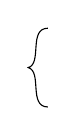
\begin{tikzpicture}[x=1cm,y=1cm]
\draw (0.25,1.1) .. controls (0,1.1) and (0.18,0.65) .. (0,0.6) .. controls (0.18,0.55) and (0,0.1) .. (0.25,0.1);
\end{tikzpicture}}

On en conclut, grâce au lemme des 5

a) $R^if_*(\mathcal O_X^*)_y\longrightarrow\varprojlim_n H^i(X_n,\mathcal O_{X_n}^{\unsure{*|\wedge}})$ est \uline{injectif}, et les \inserted{\unsure{deux mb ont $=$ images dans} $H^i(X_n,\mathcal O_{X_n}^*)$}

b) \unsure{Pour|Pourvu}

\uline{Corollaire} 1.6. \deleted{Supposons} que $R^if(\mathcal O_X)_y$ soit artinien, i.e. $y$ un pt isolé du supp $R^if(\mathcal O_X)$.
\deleted{Alors}\inserted{de sorte que}
\[
\inserted{\varinjlim_{U\ni y}H^i(f^{-1}(U),\mathcal O_U^*)=}
R^if_*(\mathcal O_X^{\unsure{*|\wedge}})\longrightarrow\varprojlim H^i(X_n,\mathcal O_{X_n}^{\unsure{*|\wedge}})
\]
soit un \uline{isomorphisme}.

\margin{\deleted{Comme le système projectif des}}
\margin{\unsure{Automatique} : pour $\unsure{n|i}$ grand \unsure{Niveau fini} $(X_0)$ est constant cad \unsure{inj} :
$\operatorname{Ker}(H^{i+1}(X_0,\mathbb Z)\longrightarrow R^{i+1}f_*(\mathcal O_X)_y)$}
\figure{\begin{tikzpicture}[x=1cm,y=1cm]
\draw (0,0) -- (0,2.5);
\draw[->] (-0.65,0.25) .. controls (-1.05,0.05) and (-0.8,-0.2) .. (-0.65,0.25);
\end{tikzpicture}}

c) \deleted{\unsure{Réciproquement}} Le lemme des 5 montre également que $R^if_*(\mathcal O_X^{\unsure{*|\wedge}})\longrightarrow\varprojlim H^i(X_n,\mathcal O_{X_n}^{\unsure{*|\wedge}})$ est toujours un \unsure{monomorphisme}.

\inserted{$\forall\xi\in\varprojlim H^i(X_n,\mathcal O_{X_n}^{\unsure{*|\wedge}})$, il existe un}
\deleted{des $(\unsure{H^i|R^i}(X_n,\mathcal O_{X_n}^*))_n$ \unsure{satisfont} M.L. (A.R.) \unsure{syst. proj.} \deleted{Comme les}}
\margin{Comme $v^{i+1}$ est injectif, $\operatorname{Ker}\alpha^{i+1}=\operatorname{Ker}\widehat\alpha^{i+1}$, \deleted{\unsure{pour}} donc $\operatorname{Im}\widehat\delta^i=\operatorname{Im}\delta^i$ donc pour}

\margin{\figure{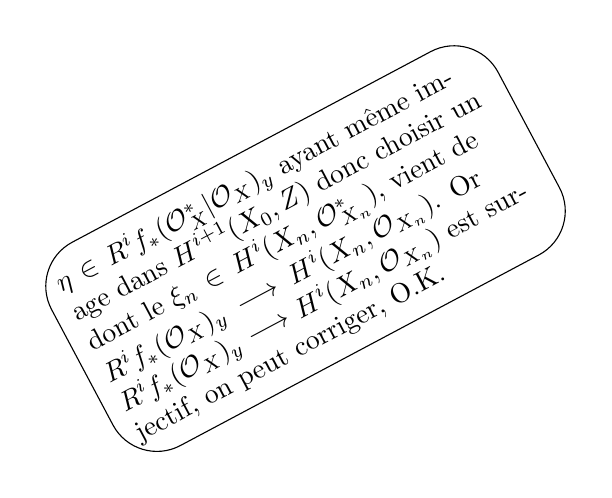
\begin{tikzpicture}
\node[draw,rounded corners=18pt,text width=6cm,align=left,rotate=28,inner sep=6pt] {
$\unsure{\eta}\in R^if_*(\unsure{\mathcal O_X^*|\mathcal O_X})_y$ ayant même image dans $H^{i+1}(X_0,\mathbb Z)$ \unsure{donc choisir un} \unsure{dont le} $\unsure{\xi_n}\in H^i(X_n,\mathcal O_{X_n}^*)$, \unsure{vient de}
\(R^if_*(\mathcal O_X)_y\longrightarrow H^i(X_n,\mathcal O_{X_n})\).
\uuline{Or} $R^if_*(\mathcal O_X)_y\longrightarrow H^i(X_n,\mathcal O_{X_n})$ est surjectif, on peut corriger, O.K.
};
\end{tikzpicture}}}

Le cas le plus important pour nous est celui où $i=1$, qui donne le

\uline{Th.} 1.\deleted{\unsure{8}}\inserted{7}. Soit $f:X\longrightarrow Y$ une application propre d'espaces analytiques sur $\mathbb C$, $y\in Y$, \inserted{$Y_n=\operatorname{Specan}\mathcal O_y/\mathfrak m_y^{n+1}$,} $X_n=X\times_Y Y_n$, \deleted{Alors} posons
\[
\operatorname{Pic}(X_y)=\varinjlim_{U\ni y}\operatorname{Pic}(f^{-1}(U))
=R^1f(\mathcal O_X^{\unsure{*|\wedge}})_y,
\]
\deleted{Alors considérons l'hom}
\[
\operatorname{Pic}(\widehat X_y)=\varprojlim_n\operatorname{Pic}(X_n).
\]
\mspage{255}

\scanpage{257}
9) L'espace des sous-groupes d'un groupe localement compact : sera distribué d'ici le Congrès.

10) Fascicule de résultats des variétés : sera distribué d'ici le Congrès.

Apporter tout ce qui pourra être distribué d'ici le Congrès.

\uline{Participants prévus} :

Borel, Bruhat, Cartier, Cartan, Dieudonné, Dixmier, Douady, Eilenberg, Godement, Koszul, Lang, Samuel, Schwartz, Serre, Weil.

Prévenir d'urgence Dixmier en cas d'erreur dans cette liste.

\begin{center}-:-:-:-\end{center}
\mspage{256}

\scanpage{258}
Considérons l'hom canonique
\[
\varphi:\operatorname{Pic}(X_y)\longrightarrow\operatorname{Pic}(\widehat X_y)
\]
(i) Le syst. projectif $(\operatorname{Pic}(X_n))_{n\in\mathbb Z}$ satisfait M.L.

\inserted{(ii) $\operatorname{Pic}(X_y)$ et $\operatorname{Pic}(\widehat X_y)$ ont $=$ image dans $\operatorname{Pic}(X_n)$, $\unsure{\forall n|\varphi}$.}

(iii) Pour que $\varphi$ soit \unsure{surjectif}, il f. et s. que $y$ soit un pt isolé du supp $R^1f_*(\mathcal O_X)$ \deleted{\unsure{en $y$}}.

(Cette condition est vérifiée en particulier si $X|(Y-\{y\})\longrightarrow Y-\{y\}$ est un isom.).

\margin{\unsure{Pour tout $n$}, de façon plus précise, $\exists k$ tel que \deleted{\unsure{les}} $H^1(X_{n+k},\mathcal O_{X_{n+k}}^*)$ et $R^1f_*(\mathcal O_X^*)_y$ aient $=$ image dans $H^1(X_n,\mathcal O_{X_n}^*)$}
\figure{\begin{tikzpicture}[x=1cm,y=1cm]\draw (0,0)--(0,4);\end{tikzpicture}}
\margin{\deleted{\unsure{Corollaire}}}

\deleted{\uline{Corollaire} 1.10 \deleted{Supposons que les} \deleted{\unsure{des espaces analytiques}} les $X_n$ soient ``algébrisables'', \deleted{et donc} se proviennent de schémas propres $\mathfrak X_n$ sur les $\mathfrak Y_n=\operatorname{Spec}\mathcal O_y/\mathfrak m_y^{n+1}$. Soit $\mathfrak X$ le schéma formel propre sur $\widehat{\mathcal O}_y$ défini par le système inductif des $\mathfrak X_n$. Supposons \deleted{de plus} \deleted{que $\mathfrak X$ sur $\widehat{\mathcal O}_y$ soit} que $y$ soit un pt isolé de $R^1f(\mathcal O_X)$.

\deleted{Deux} Conditions équivalentes :

(i) Il existe un voisinage ouvert $U$ de $y$ tel que $X|U$ soit projectif sur $U$ (\deleted{\unsure{Séminaire}} \unsure{Sém.} Cartan 1960/61).

(ii) \deleted{$\unsure{\mathfrak X}$ \illegible{2}}

b) \deleted{$\mathfrak X$ est algébrisable}}
\figure{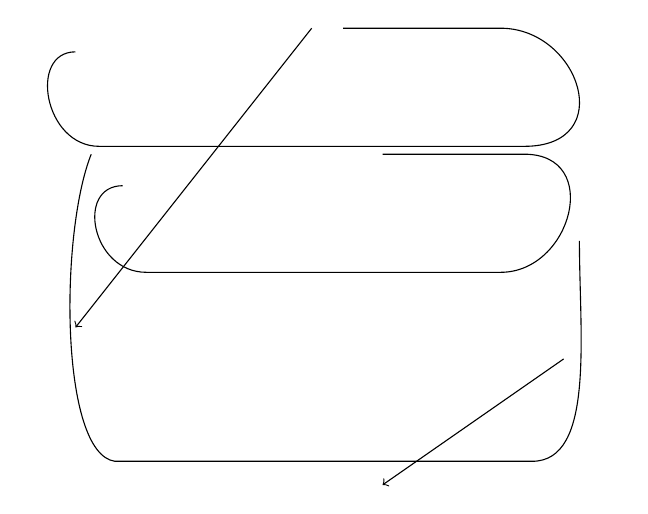
\begin{tikzpicture}[x=1cm,y=1cm]
\draw (0.1,5.5) .. controls (-0.5,5.5) and (-0.3,4.3) .. (0.4,4.3) -- (5.8,4.3) .. controls (7,4.3) and (6.5,5.8) .. (5.5,5.8) -- (3.5,5.8);
\draw (0.7,3.8) .. controls (0.1,3.8) and (0.3,2.7) .. (1,2.7) -- (5.5,2.7) .. controls (6.4,2.7) and (6.8,4.2) .. (5.8,4.2) -- (4,4.2);
\draw (0.3,4.2) .. controls (-0.1,3.2) and (-0.1,0.4) .. (0.6,0.3) -- (5.9,0.3) .. controls (6.7,0.3) and (6.5,1.9) .. (6.5,3.1);
\draw[->] (3.1,5.8) -- (0.1,2);
\draw[->] (6.3,1.6) -- (4,0);
\end{tikzpicture}}
\mspage{257}

\scanpage{259}
\begin{center}\uline{B O U R B A K I ' S\quad D I K T Ä T}\end{center}

Le prochain Congrès se tiendra du Lundi 25 juin au Samedi 7 juillet à Aiguines (Var), Auberge Relais, (tél. 9).

Pour les parisiens, départ le Dimanche 24 à 22 h 13, gare de Lyon, par le train autos-couchettes. Arrivée à Avignon à 7 h 23. Les voitures de Serre, Samuel, Bruhat emmèneront les voyageurs d'Avignon à Aiguines. Il est presque indispensable d'effectuer en même temps la location voiture et l'achat des billets aller et retour des voyageurs. Chacun est donc prié d'envoyer \uline{d'urgence} à Dixmier ses intentions précises concernant le voyage aller et le voyage retour.

Pour ceux qui n'utiliseront pas la méthode précédente, la moins mauvaise solution consiste à prendre le train jusqu'à Toulon, puis un car Toulon-Aups, puis un car Aups-Aiguines.

\uline{Programme} :

1) Algèbre commutative. Chap. VII, Diviseurs, § 4, Modules sur les anneaux intégralement clos, n° 353. (Apporter le n° 300, rapport d'Arithmétique. Samuel apportera une documentation).

2) La ramification dans les corps locaux (rédaction tirée en noir à Paris). Apporter le n° 363, (démonstration du théorème de Hasse-Arf).

3) ``Un bout de rédaction'' (il s'agit de la théorie de Morse). (Rédaction tirée en noir à Paris).

4) Algèbre, réédition du chap. III, n° 371, (Koszul apportera les épreuves de la réédition du chap. II).

Algèbres cayleyennes : n° 381.

5) Une rédaction sur les groupes de Lie qui doit être distribuée avant le Congrès. Apporter le n° 372 (Variétés de groupes ; groupes standard et applications) et le n° 340 (Variétés de groupes).

\margin{\figure{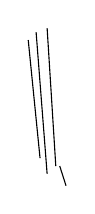
\begin{tikzpicture}[x=1cm,y=1cm]
\draw (0,1.7)--(.15,.2);\draw (.1,1.8)--(.24,0);\draw (.24,1.85)--(.35,.1);\draw (.4,.1)--(.48,-.15);
\end{tikzpicture}}}
6) Une rédaction sur les systèmes de racines qui doit être distribuée prochainement. Apporter le n° 351, et le papier de Tits (Groupes et géométries de Coxeter) tiré en noir à l'IHES.

7) Existence de représentations intégrales dans les convexes compacts : n° 379. Apporter le n° 378.

8) Algèbres normées, n° 380. Dixmier apportera une documentation.

\mspage{258}

\scanpage{260}
\uline{Corollaire} 1.8. Soit $f:X\to Y$ un morphisme propre d'espaces analytiques \inserted{sur $\mathbb C$}, et $y\in Y$. Conditions équivalentes :

(i) $\exists$ un voisinage ouvert $U$ de $y$ tel que $X|U$ soit \uline{proj} sur $U$ (cf Sém. Cartan).

(ii) Pour tout entier $n$, $X_n=X\times_Y Y_n$ (i.e. $Y_n=\operatorname{Specan}\mathcal O_y/\mathfrak m_y^{n+1}$) est \deleted{\unsure{proj}} un espace analytique projectif.

\uline{Dém}. Réf : Sém. Cartan ....

Exemple

\margin{\figure{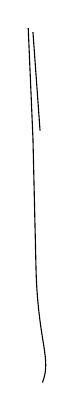
\begin{tikzpicture}[x=1cm,y=1cm]\draw (0,4.5)--(.06,3.1)--(.1,1.4)..controls(.13,.5)and(.3,.3)..(.18,0);\draw (.06,4.45)--(.15,3.2);\end{tikzpicture}}}
\uline{Corollaire} \deleted{\unsure{1.8|1.9}} 1.9. \deleted{Supposons} Soit $f:X\unsure{-|\to}Y$ un morphisme propre d'espaces analytiques sur $\mathbb C$, \deleted{\unsure{et} tel que \unsure{dim|les} $\unsure{X_y}$} dont les fibres soient de dim $\leq 1$. Alors $f$ est localement projectif.

Résulte du

\uline{Lemme} 1.9. Un espace analytique compact de dim $\leq 1$ est projectif.

\mspage{259}

\scanpage{261}
\mspage{7}
\margin{n° 324}
Cette fonctions est \uline{dérivable} en $x_0$, et sa dérivée est donnée par la formule :
\[
(7)\quad (f_1\cdot f_2)'(x_0)\cdot h=(f'_1(x_0)\cdot h)\cdot f_2(x_0)+f_1(x_0)\cdot(f'_2(x_0)\cdot h),\quad h\in E,
\]
formule que l'on écrit aussi plus brièvement :
\[
(7\text{ bis})\quad (f_1\cdot f_2)'(x_0)=f'_1(x_0)\cdot f_2(x_0)+f_1(x_0)\cdot f'_2(x_0),
\]
ou même :
\[
(7\text{ ter})\quad (f_1\cdot f_2)'=f'_1\cdot f_2+f_1\cdot f'_2.
\]
Ceci s'applique notamment lorsque $F_1=F_2=F=K$ (fonctions à valeurs scalaires).

f). \uline{Théorème des fonctions implicites}. Les notations étant celles de b), on suppose que $E$ et $F$ sont \uline{normés} et \uline{complets} (ce qui est toujours le cas lorsque $E$ et $F$ sont de dimension finie, cf. EVT, chap. I, § 2), que $f$ est \uline{strictement dérivable} au point $x_0$, et que $f'(x_0):E\longrightarrow F$ est un \uline{isomorphisme} d'espaces vectoriels topologiques. Soit $y_0=f(x_0)$. Il existe alors $^{(3)}$ une application $g$ d'un voisinage de $y_0$ dans $E$, strictement dérivable en $y_0$, prenant la valeur $x_0$ en ce point, et telle que $g\circ f=1_E$ (resp. $f\circ g=1_F$) au voisinage de $x_0$ (resp. de $y_0$).$^{(4)}$

g) \uline{Dérivées partielles}. On suppose maintenant que $E=K^n$ ; soit $x_0=(x_1^0,\ldots,x_n^0)\in E$. La fonction $f:U\to F$ peut donc être considérée comme une fonction $f(x_1,\ldots,x_n)$ de $n$ variables scalaires, à valeurs dans $F$, définie lorsque les $x_i$ sont assez voisins des $x_i^0$. Si on laisse les $x_j$ fixes, égaux à $x_j^0$, pour tout $j\neq i$, on obtient une fonction de la seule variable $x_i$, définie au voisinage de $x_i^0$.

\mspage{260}

\scanpage{262}
Démonstration calquée sur celle qui \unsure{sert|sort} dans le cas algébrique, \unsure{utilisant} RR analytique ....

\uline{Remarque} 1.10. Bien entendu, sous les conditions 1.8 \inserted{(ou de 1.9.)} on ne peut en général conclure que $f$ est projectif (globalement). Il en est cependant ainsi dans le cas suivant :

\figure{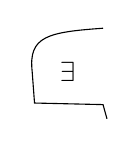
\begin{tikzpicture}[x=1cm,y=1cm]\node at(.45,.4){$\exists$};\draw (.9,.95)..controls(.2,.9)and(-.05,.85)..(0,.4)--(.03,0)--(.9,-.02)--(.95,-.2);\end{tikzpicture}}
partie discrète $T$ de $Y$ telle que

a) $X|(Y-T)\longrightarrow Y-T$ est \deleted{\uline{fini}} un isom

b) les anneaux locaux $\mathcal O_y$ $(y\in T)$ sont factoriels.

En effet, dans ce cas il est facile de construire un sous-\deleted{\unsure{ensemble}}\inserted{espace} analytique fermé $Z$ de $Y$, \uline{de support $\subset T$}, tel que $X$ soit $Y$-isom. à l'espace analytique \unsure{``déduit de $Y$'' en ``faisant éclater'' $Z$''}.

\uline{Remarque} 1.11. Sur les \unsure{variantes} analytique-formelle et algébrique formelle du th. envisagé. Il y a pour cette dernière une démonstration purement algébrique, utilisant \uline{Pic}, \deleted{\unsure{et}}\inserted{et} th. de finitude de Néron.

\mspage{261}

\scanpage{263}
\mspage{44}
\margin{n° 227}
linéaires.

Soit $\unsure{\mathcal P|\mathcal S}$ un pencil. Un point $P'$ de $V$ est un \uline{point de base de} $\mathcal P$ si $P'\in|X|$ pour tout $X\in\mathcal P$.

THÉORÈME 3. -- \uline{Soit} $\mathcal P$ \uline{un pencil de genre} $\geq1$. \uline{Alors} $\mathcal P$ \uline{n'a pas de points de base qui soit simple sur} $V$.

\uline{Dém}. On va se servir d'un peu de variétés abéliennes ; Soit $k$ un corps de rationalité pour $V$, $\mathcal P$ et $P'$, et soit $f:V\longrightarrow C$ la fonction définissant $\mathcal P$. Soit $Q$ un point générique de $C/k$ et $P$ un point générique de $V$ tel que $f(P)=Q$. Alors on voit que $P'$ est une spécialisation de $P$ sur $k(Q)$, parce que $P'$ est un point dans le cycle premier rationnel ayant $P$ comme point générique sur $k(Q)$. Mais $P'$ étant rationnel sur $k$, on voit que la fonction $f$ ne peut être définie en $P'$. On peut supposer que $C$ est plongée dans sa Jacobienne. Ceci contredit le théorème 6 de VA.

\mspage{262}

\scanpage{264}
§ 2 Application à la géométrie algébrique sur une algèbre analytique.

\uline{Th}. 2.1. Soient $A$ une algèbre analytique sur $\mathbb C$, \inserted{$Y=\operatorname{Spec}A$,} $X$ un schéma propre sur $A$, \deleted{Alors} $\widehat Y=\operatorname{Specf}\widehat A$, $\widehat X=X\times_Y\widehat Y$, \deleted{Alors} de sorte que [cf] \deleted{$\unsure{\varphi}$} $\operatorname{Pic}(\widehat X)\simeq\varprojlim\operatorname{Pic}(X_n)$.

Alors

a) $(\operatorname{Pic}(X_n))_n$ satisfait ML

\margin{se généralise aux \uline{\unsure{schémas}} formels en \uuline{car. 0}
\figure{\begin{tikzpicture}[x=1cm,y=1cm]\draw[<->] (0,0)--(2.7,.7);\end{tikzpicture}}}

(ii) $\operatorname{Pic}(X)$ et $\operatorname{Pic}(\widehat X)$ ont $=$ image dans $\operatorname{Pic}(X_{\unsure{0|n}})$.
[\unsure{donc les comp. universelles|donne les comp. universelles}]

(iii) Pour q
\[
\varphi:\operatorname{Pic}(X)\unsure{-|\to}\operatorname{Pic}(\widehat X)
\]
soit un isom il faut s. que $H^1(X,\mathcal O_X)$ soit de longueur finie sur $A$, i.e. $\operatorname{supp}R^1f_*(\mathcal O_X)\subset\{y\}$ ($y$ le pt fermé de $Y$), \deleted{\unsure{ce qui équivaut|ce qui implique} \inserted{\unsure{le groupe}} \unsure{de} \unsure{isomorphisme} \unsure{que le syst.} projectif $(\operatorname{Pic}(X_n))$ soit ess\textsuperscript{t}. constant}
\figure{\begin{tikzpicture}[x=1cm,y=1cm]
\draw (0,0)--(2.5,.8)--(5.2,1.3)..controls(6,1.4)and(6.6,1.3)..(7,1.3)..controls(7.3,1.2)and(7.2,.8)..(7.8,.65)--(10,.7)--(10.5,.5)--(10.4,-.1)--(0,-.2)--(0,0);
\draw (0,.1)--(9.5,1.1);\draw (0,-.1)--(10.5,.5);
\draw (0,0)..controls(.8,-.4)and(1.1,.9)..(1.2,.2)..controls(1.5,-.2)and(1.8,.4)..(2,.9)..controls(2.2,-.4)and(2.5,-.1)..(2.7,.1)--(3.2,1)..controls(3.4,-.3)and(3.8,.1)..(4.1,.7)..controls(4.3,-.3)and(4.7,-.2)..(5,.3)--(5.2,1.2)..controls(5.3,-.2)and(5.8,.5)..(6,1.1)..controls(6.3,.3)and(6,.0)..(6.8,.1)--(7.5,.9)..controls(7.6,-.1)and(8.2,-.1)..(8.6,.0)--(8.5,.8)--(9.1,.2)--(9.8,-.1)--(10.2,.5);
\draw (5.3,1.2) ellipse (.9,.25);
\end{tikzpicture}}

Notons de suite le corollaire suivant de \deleted{l'injectivité de} a) et ii)

\uline{Corollaire} 2.2. Conditions équivalentes

\mspage{263}

\scanpage{265}
\mspage{12}
\margin{n° 227}
normale) la fonction $f_i z$ est définie à chaque point de $V_i$, et induit donc une fonction $f'_i z'$ sur $W$ ou $W^*$, définie à chaque point de $W$ ayant un représentant sur $V_i$. Si $V'_i$ est le représentant affine de $W$ dérivé de $V_i$, on voit par ce qui précède que les pôles de $z'$ ayant un représentant sur $V'_i$ sont bornés par les zéros de $f'_i$. La variété $W$ étant couverte par un nombre fini de ces variétés affines, on voit que les pôles de $z'$ sont uniformément bornés, cqfd.

Revenons à la démonstration du théorème. Sachant que $L(0)=k$, il suffit de montrer que si le théorème est vrai pour un diviseur positif $D$, alors pour tout diviseur premier $W$, $L(D+W)$ est de dimension finie.

Supposons que $W$ apparaisse avec la multiplicité $n$ dans $D$, i.e. $D=nW+\ldots$. S'il n'y a pas de fonction $f\in L(D+W)$ ayant un pôle d'ordre $n+1$ sur $W$, alors $L(D+W)=L(D)$, et nous avons fini. Autrement, supposons qu'il existe une fonction $f$ dans $L(D+W)$ ayant un pôle d'ordre $n+1$ sur $W$. Considérons l'espace vectoriel $f^{-1}L(D+W)$, formé de tous les produits $f^{-1}g$, avec $g\in L(D+W)$. Il est évidemment égal à $L(D+W+(f))$. Aucune des fonctions de cet espace n'a de pôle sur $W$. Par conséquent chacune de ces fonctions induit une fonction sur $W$, et on a un homomorphisme $h\longrightarrow h'$ où $h\in L(D+W+(f))$, et $h'$ est la fonction induite sur $W$. Le lemme, et l'hypothèse d'induction, montrent que l'image de notre homomorphisme est de dimension finie.

Si une fonction $f^{-1}g$ induit la constante $0$ sur $W$, alors $f^{-1}g$ a un zéro sur $W$, et $g$ a donc un pôle d'ordre au plus $n$ sur $W$. Mais $g$ étant dans $L(D+W)$, on voit que $g$ est même dans $L(D)$. Le noyau de notre homomorphisme est donc précisément l'espace $L(D)$, qui est

\mspage{264}

\scanpage{266}
\unsure{a)|(i)} $X$ est projectif sur $Y$

(ii) $\widehat X$ est projectif sur $\widehat Y$, i.e. $X\otimes_A\operatorname{Spec}(\widehat A)$ projectif sur $\operatorname{Spec}\widehat A$

(iii) Pour tout entier $n$, $X_n$ est projectif sur $Y_n$.

Évident $\text{a)}\Rightarrow\text{(ii)}\Rightarrow\text{(iii)}$. Prouvons $\text{(iii)}\Rightarrow\text{a)}$. Soit $n_0$ tel que l'image de $\operatorname{Pic}(X_{n_0})\unsure{-|\to}\operatorname{Pic}(X_0)$ soit universelle.

Soit $L_{n_0}$ Module inv. sur $X_{n_0}$ ample $/Y_{n_0}$. \deleted{\unsure{Il|Je} provient d'un $\unsure{L}$} \inserted{Donc $\unsure{L_0|L}$ en vertu de 2.1. (i)} provient d'un module inv. $\mathcal L$ sur $\widehat X$, donc en vertu de \deleted{\unsure{(i)}} 2.1. (ii) il provient aussi d'un module \inserted{inv.} $L$ sur $X$. Ce dernier est ample en vertu de EGA III. Qfd.

\margin{$L_0=L_{n_0}|X_0$
\figure{\begin{tikzpicture}[x=1cm,y=1cm]\draw (0,1)..controls(1,1.5)and(2,1.2)..(2.2,.5)--(2.15,-.1)--(.8,-.1)..controls(.35,-.2)and(.7,-.55)..(.1,-.5);\end{tikzpicture}}}

Notons maintenant que 2.1. \deleted{\unsure{(i)}} se déduit aisément de 1.7. par le \unsure{Gaga|Gag} de Serre-Grauert-Remmert-Grothendieck

\mspage{265}

\scanpage{267}
\mspage{11}
\margin{n° 227}
$n$ sur $Q$. Mais $z-aw$ est dans $L(D+Q)$, donc dans $L(D)$. Ceci contredit l'indépendence linéaire de $z$ et $w$ mod $L(D)$.

Supposons maintenant le théorème démontré pour toutes les variétés de dimension $<r$. On va procéder par induction. Faisons d'abord quelques remarques. Soit $z$ une fonction sur $V$, et $W$ un diviseur premier de $V$. Alors $W$ n'est pas nécessairement normale. Soit $P'$ un point générique de $W$. Alors la spécialisation $P\longrightarrow P'$ induit une place du corps $k(P)$. Si la fonction $z$ n'a pas de pôle sur $W$, elle est dans l'anneau de valuation de cette place et est définie sur $W$. Son image $z'$ dans le corps $k(P')$ définit une fonction sur $W$. La normalisation $W^*$ de $W$ ayant le même corps de fonction que $W$, on peut dire que si $z$ n'a pas de pôle sur $W$, alors $z$ induit sur $W$ ou sur $W^*$ une fonction $z'$. C'est de cette fonction qu'il s'agira dans le lemme suivant.

LEMME. -- \uline{Soit} $D$ \uline{un diviseur sur} $V$, \uline{et} $W$ \uline{un diviseur premier de} $V$, \uline{non contenu dans les composantes polaires de} $D$. \uline{Alors il existe un diviseur} $D^*$ \uline{sur la normalisation} $W^*$ \uline{de} $W$ \uline{tel que pour une fonction} $z\in L(D)$, \uline{la fonction induite} $z'$ \uline{sur} $W^*$ \uline{soit dans} $L(D^*)$.

\uline{Dém}. Soit $V_i$, $i=1,\ldots,g$ les représentants de $V$. On peut supposer que tous les $V_i$ sont des variétés affines. D'après un théorème d'approximation élémentaire, il existe une fonction $f_i\in K$ telle que pour $z\in L(D)$, la fonction $f_i z$ n'ait pas de pôle ayant un représentant sur $V_i$, et telle que $f_i$ soit une unité sur $W$.

Si $W$ a un représentant sur $V_i$, alors les fonctions $f_i$, $z$, et $f_i z$ sont définies sur $W$, et induisent des fonctions $f'_i$, $z'$ et $f'_i z'$ sur $W$. De plus, $\unsure{f'_j|f'_i}\neq0$. Alors, d'après la prop.5 ($V$ étant supposée

\mspage{266}
